\documentclass{article}
\usepackage{nips15submit_e,times}
\usepackage{hyperref}
\usepackage{url}
\usepackage{amsmath}
\usepackage{amsfonts,amssymb}
\usepackage{graphicx}

\title{Weekly Report(July.9,2018-July.15,2018)}

\author{Zhang Yuandi}

\newcommand{\fix}{\marginpar{FIX}}
\newcommand{\new}{\marginpar{NEW}}

\begin{document}


\maketitle

\begin{abstract}
In the last week, I learned week2, week3, week4 of \textbf{Machine Learning}. To know more about js, I learned \textbf{HTML, CSS, and Javascript for Web Developers} on coursera and implemented the basic function of \emph{wordladder.js}. About data structure, I learned B-Tree. What's more, I have my initial time with Object Detection Networks.

\end{abstract}
\section{Work done in this week}
\subsection{Machine Learning}
\subsubsection{Environment Setup}
Thanks for free access to MATLAB, I can use it to do powerful works. However, I tried Octave Professor Ng recommended, but got stuck when graphing. When I use the function \emph{hist()} in Octave GUI, the outcome is just like this:
\begin{center}

\includegraphics[scale=0.6]{mistake.png}
\end{center}
Then I searched for some methods trying to fix it, like downloading \emph{gnuplot}, which runs well on my computer, like changing \emph{graphics$\_$toolkit}:
\begin{center}
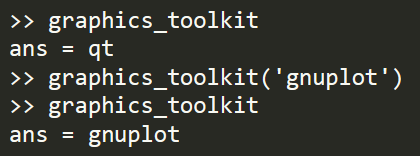
\includegraphics[scale=0.6]{m.png}
\end{center}
But this problem of graphing still exists, which makes me feel dizzy. Luckily, MATLAB works well.

\subsubsection{Multivariate Linear Regression}
It's a common sense that numerous objects have multiple features, so we ought to facilitate our algorithm. We get these:
\begin{itemize}
  \item Hypothesis: $h_{\theta}(x) = \theta^Tx = \theta_0x_0 + \theta_1x_1 + \theta_2x_2 + \cdots + \theta_nx_n$
  \item Parameters: $\theta_0, \theta_1, \ldots, \theta_n$
  \item Cost Function: $J(\theta_0, \theta_1, \ldots, \theta_n) = \frac{1}{2m}\sum_{i=1}^m(h_{\theta}(x^{(i)}-y^{(i)})^2)$
  \item Gradient Descent($n \geq 1$): Repeat\{ \[\theta_j := \theta_j - \alpha\frac{1}{m}J(\theta_0, \theta_1, \ldots, \theta_n)x_j^{(i)}\]\}(simultaneously update for every $j = 0, \ldots, n$)
\end{itemize}

\subsubsubsection{Feature Scaling}\\
To make sure features are on the same scale, we can get every feature into approximately a $-1 \leq x_i \leq 1$ range by mean normalization:
\begin{center}
Replace $x_i$ with $\frac{x_i - \mu_i}{s_i}$ ($\mu_i$ is the average of $x_i$ and $s_i$ = max - min)
\end{center}

\subsubsubsection{Learning Rate}\\
How to make sure gradient descent is working correctly?\\
We declare convergence if $J(\theta)$ decreases by less than 10$^{-3}$ in one iteration.
\begin{itemize}
\item If $\alpha$ is too small, the convergence will be very slow.
\item If $\alpha$ is too large, $J(\theta)$ may not decrease on every iteration; may not convergence.
\end{itemize}
When the outcome of our convergence looks strange, then we need to choose a better $\alpha$.

\subsubsubsection{Normal Equation}\\
Normal Equation is a method to solve for $\theta$ analytically. We declare:
\[X = \left (\begin{array}{c}
                (x^{(1)})^T \\
                (x^{(2)})^T \\
                \vdots \\
                (x^{(m)})^T
              \end{array}\right) \]
Then we have \[\theta = (X^TX)^{-1}X^Ty\]
We can make a simple comparison between Gradient Descent and Normal Equation.
\begin{table}[h]
\centering
\begin{tabular}{|c|c|}
\hline
Gradient Descent & Normal Equation \\ \hline
   Need to choose $\alpha$. & Don't need to choose $\alpha$. \\
   Need many iterations. & Don't need to iterate. \\
   Works well even when n is large. & Need to compute $(X^TX)^{-1}$\\
    & Slow if n is very large.\\ \hline
\end{tabular}
\end{table}

\subsubsection{Logistic Regression}
\begin{itemize}
  \item Classification: y = 0 or 1, $h_{\theta}(x)$ can be $>$ 1 or $<$ 0
  \item Logistic Regression: $0 \leq h_{\theta}(x) \leq 1$
\end{itemize}

We make our Logistic Regression:
\[h_{\theta}(x) = g(\theta^Tx)\]
\[g(z) = \frac{1}{1+e^{-z}}\]
\[Cost(h_{\theta}, y) = \begin{cases}
-log(h_{\theta}(x)) & \text{if y = 1}\\
-log(1 - h_{\theta}(x)) & \text{if  y = 0}
\end{cases}\]

\subsubsubsection{Gradient Descent}\\
\[J(\theta) = -\frac{1}{m}[\sum_{i=1}^{m}y^{(i)}logh_{(\theta)}(x^{(i)}) + (1 - y^{(i)})log(1 - h_{\theta}(x^{(i)}))]\]
Want min$_{\theta}$ $J(\theta)$:\\
Repeat\{ \[\theta_j := \theta_j - \alpha\sum_{i=1}^m(h_{\theta}(x^{(i)}) - y^{(i)})x_j^{(i)}\] \}

\subsubsection{Overfitting}
If we have too many features, the learned hypothesis may fit the training set very well ($J(\theta) \approx 0$ ), but fail to generalize to new examples. What can we do to fix the problem?
\begin{enumerate}
  \item Reduce number of features.
  \item Regularization.
\end{enumerate}

\subsubsection{Regularization Cost function}
\[J(\theta) = \frac{1}{m}[\sum_{i=1}{m}(h_{\theta}(x^{(i)}) - y^{(i)})^2 + \lambda\sum_{j=1}{n}\theta_j^2]\]
What if $\lambda$ is set to an extremely large value?
\begin{itemize}
  \item Algorithm works fine; setting $\lambda$ to be very large can��t hurt it.
  \item Algorithm fails to eliminate overfitting.
  \item Algorithm results in underfitting. (Fails to fit even training data well).
  \item Gradient descent will fail to converge.
\end{itemize}

\subsubsubsection{Gradient Descent}\\
Repeat\{
\[\theta_j := \theta_j(1 - \alpha\frac{\lambda}{m}) - \alpha\frac{1}{m}\sum_{i=1}^{m}(h_{\theta}(x^{(i)}) - y^{(i)})^2x_j^{(i)} \]\}
\subsubsubsection{Normal Equation}
\[\theta = (X^TX + \lambda\left(
                            \begin{array}{ccccc}
                              0 &   &   &   &   \\
                                & 1 &   &   &   \\
                                &   & 1 &   &   \\
                                &   &   & \ddots &   \\
                                &   &   &   & 1 \\
                            \end{array}
                          \right))^{-1}X^Ty
\]

\subsubsection{Neural Networks}
Actually it is a little hard to understand fully, since I have't tried it yet and think it's somehow abstract. This picture shows clearly how neural networks work:
\begin{center}
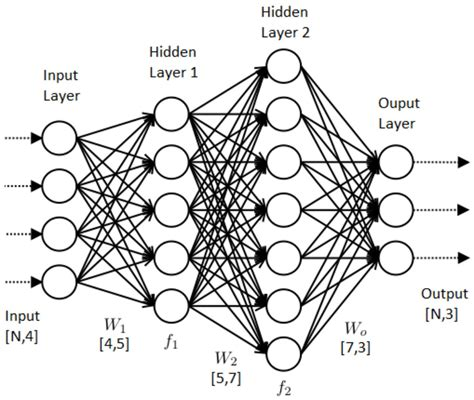
\includegraphics[scale=0.6]{3.jpg}
\end{center}
We declare that \\
$a_i^{(j)}$ = "activation" of unit i in layer j\\
$\Theta^{(j)}$ = matrix of weights controlling function mapping from layer j to layer j + 1\\
If network has $s_j$ units in layer j, $s_{j+1}$ units in layer j + 1 , then $\Theta^{(j)}$ will be of dimension $s_{j+1} \times (s_{j} + 1)$.
The steps look like this:
\[\left[
  \begin{array}{c}
    x_0 \\
    x_1 \\
    x_2 \\
    \cdots \\
    x_n \\
  \end{array}
\right]
\rightarrow
\left[
  \begin{array}{c}
    a_0^{(2)} \\
    a_1^{(2)} \\
    a_2^{(2)} \\
    \cdots \\
  \end{array}
\right]
\rightarrow
\left[
  \begin{array}{c}
    a_0^{(3)} \\
    a_1^{(3)} \\
    a_2^{(3)} \\
    \cdots \\
  \end{array}
\right]
\rightarrow
\cdots
\rightarrow
\left[
  \begin{array}{c}
    h_{\Theta}(x)_1 \\
    h_{\Theta}(x)_2 \\
    h_{\Theta}(x)_3 \\
    h_{\Theta}(x)_4 \\
  \end{array}
\right]\]

\subsection{Js}
The biggest problem I met is reading files. I solved it with the help of Ajax. Here is part of the function:
\begin{center}
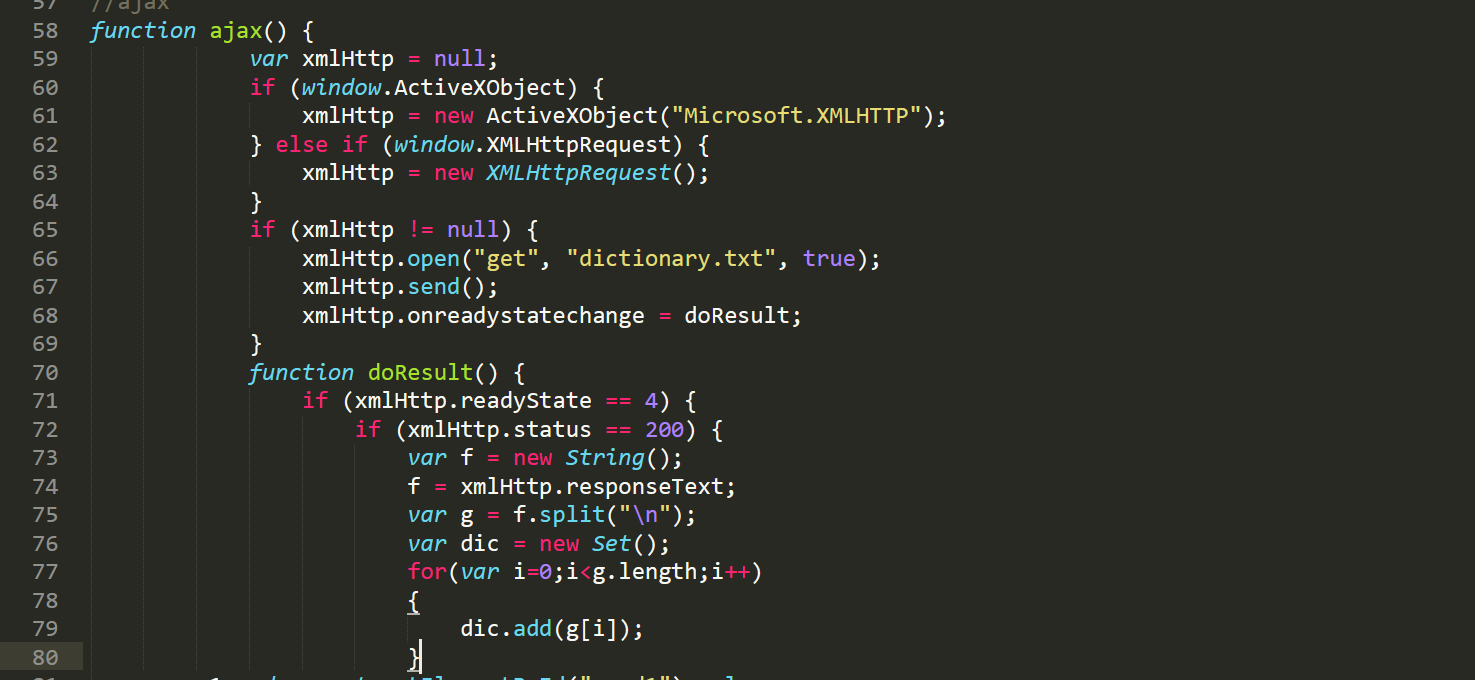
\includegraphics[scale=0.4]{5.png}
\end{center}
And the function \emph{replace()} of a string doesn't change the original string itself. Also, the shallow copy of an object should be highly paid attention.

\subsection{Data Structure}
The B$-$tree is a generalization of a binary search tree in that a node can have more than two children. It is very efficient for storage systems that read and write relatively large blocks of data, such as discs. The basic rule for a B$-$tree are as follows:
\begin{enumerate}
  \item Every node has at most m children.
  \item Every non-leaf node (except root) has at least [m/2] children.
  \item The root has at least two children if it is not a leaf node.
  \item A non-leaf node with k children contains k$-$1 keys.
  \item All leaves appear in the same level.
\end{enumerate}

\subsection{Detection Networks}
This is quite hard to understand at the beginning, but I'm trying to ignore some details and focus on the procedure. I learned some basic steps of some important detection model.

\subsubsection{R$-$CNN}
Region-based Convolutional Neural Network(R$-$CNN), consisted of 3 simple steps, which can be illustrated like this:
\begin{center}
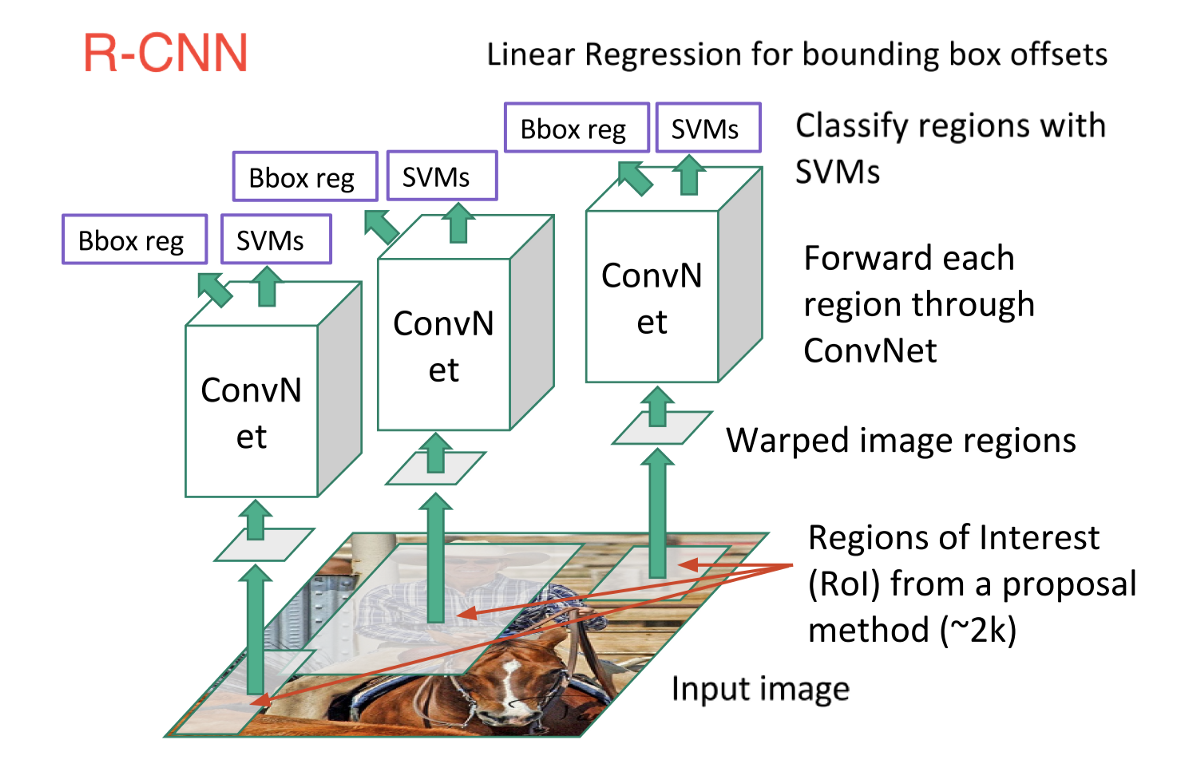
\includegraphics[scale=0.2]{7.png}
\end{center}

\subsubsection{Fast R$-$CNN}
The reason why it is fast is that we can train just one CNN for the entire image. The steps can be illustrated like this:
\begin{center}
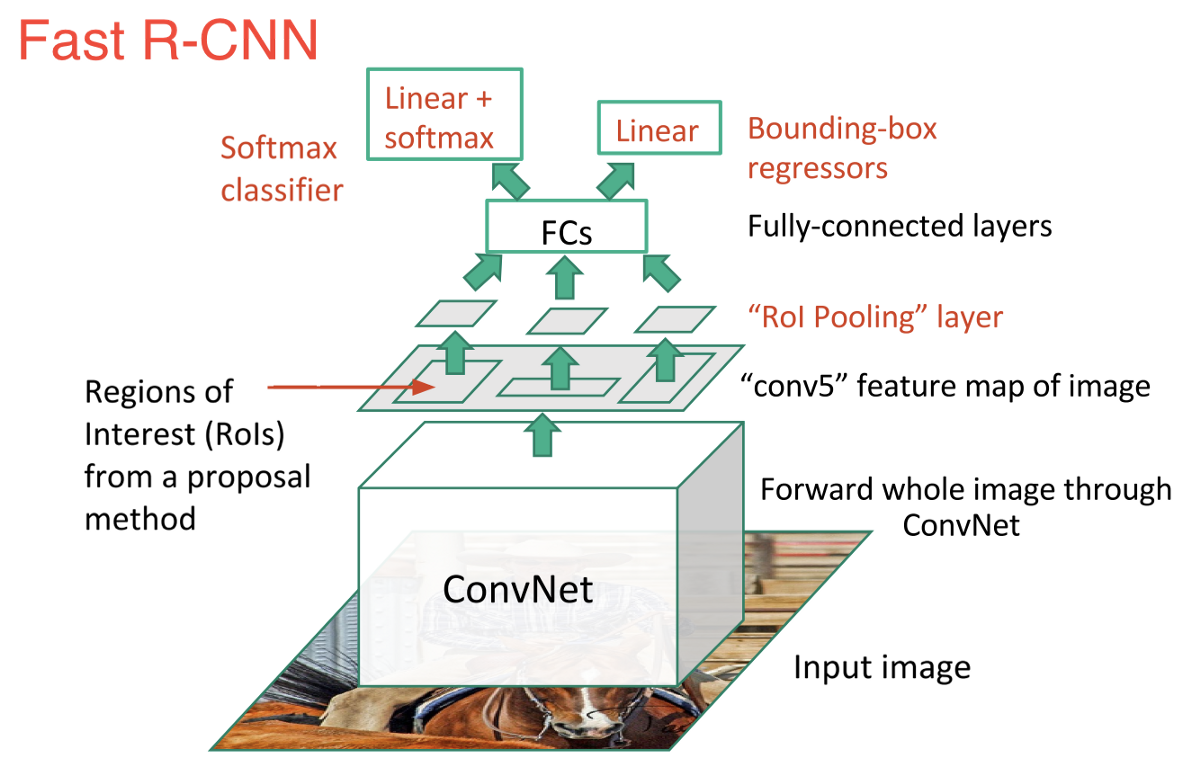
\includegraphics[scale=0.2]{8.png}
\end{center}

\subsubsection{Faster R$-$CNN}
Specifically, it introduced the region proposal network (RPN). Here is how RPN works:
\begin{center}
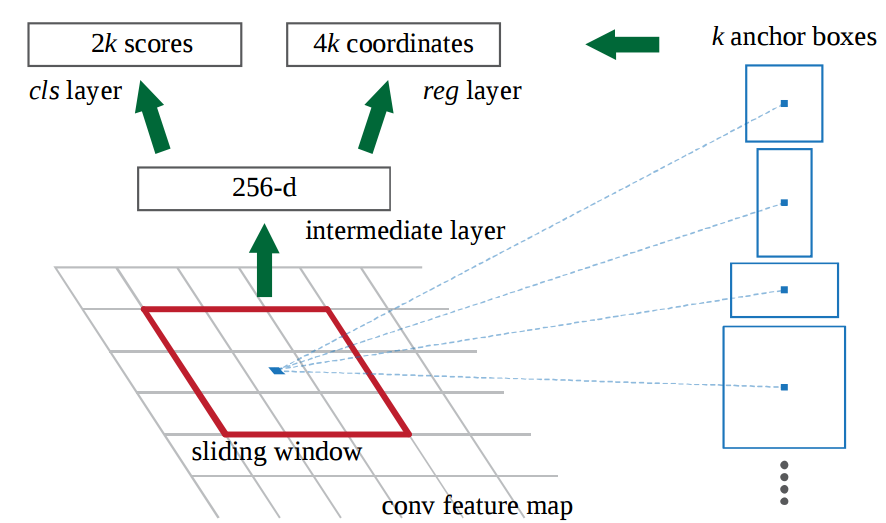
\includegraphics[scale=0.3]{9.png}
\end{center}
But to be honest, this is somehow hard to understand, at least I haven't understand it fully.
In a sense, \textbf{Faster R$-$CNN = RPN + Fast R$-$CNN}.

\subsubsection{R$-$FCN}
Region-based Fully Convolutional Net(R$-$FCN) uses the position$-$sensitive score maps, which are convolutional feature maps that have been trained to recognize certain parts of each object. to help us compromise between location and location variance. It can be illustrated like this:
\begin{center}
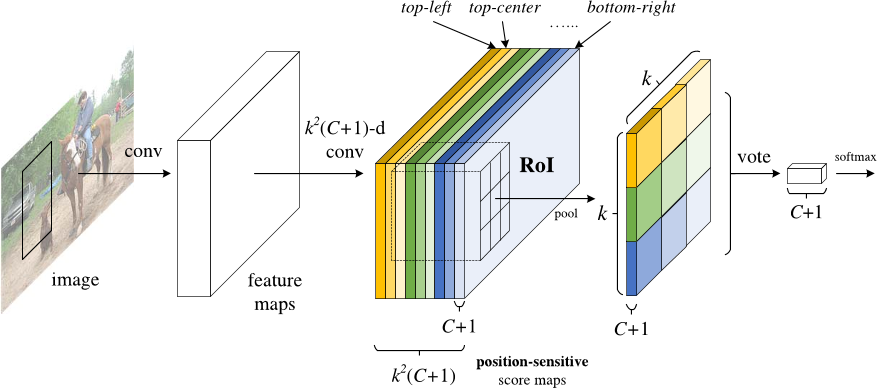
\includegraphics[scale=0.3]{11.png}
\end{center}

\subsubsection{SSD}
Single$-$Shot Detector(SSD) provides enormous speed gains over Faster R$-$CNN in a markedly different manner. SSD generates regions of interest and classifies regions in a "single shot", that is, simultaneously predicting the bounding box and the class as it processes the image. It can be illustrated like this: 
\begin{center}
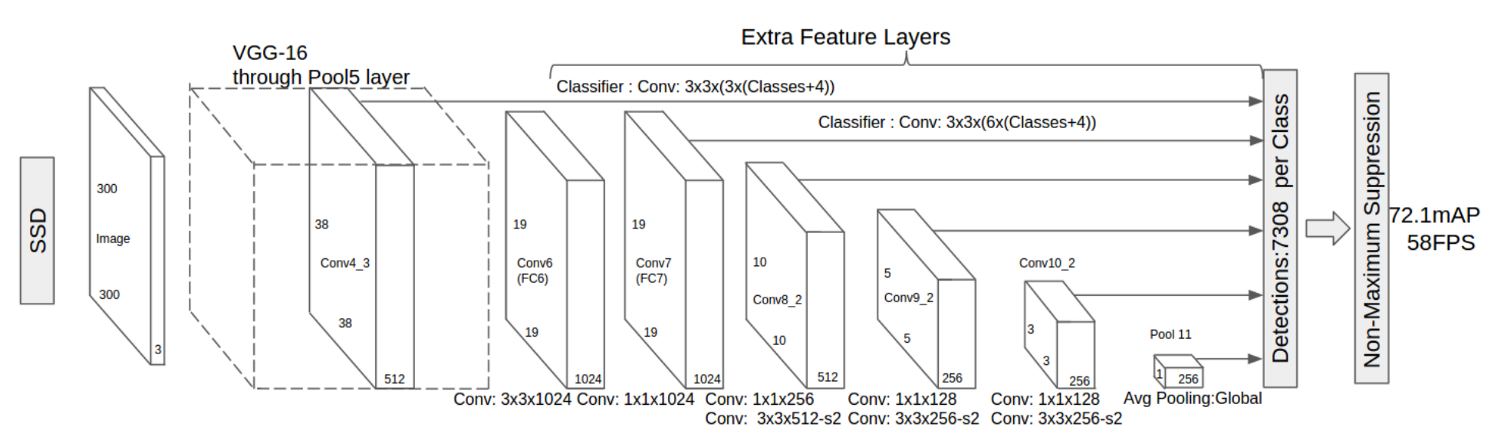
\includegraphics[scale=0.2]{13.png}
\end{center}

\section{Plans for Next Week}
\begin{enumerate}
  \item Learn the course of week5, week6, week7 of \textbf{Machine Learning}.
  \item Write a data base in C++ code.
  \item Learn more about Detection Networks.
\end{enumerate}

\end{document}
